\chapter{Implementazione}

\section{Panoramica dell'Architettura}

Il sistema Skill Manager è stato implementato con i servizi del Cloud Provider Amazon Web Services (AWS) e sostanzialmente è composto da:

\begin{itemize}
    \item Distribuzione CloudFront della Web App.
    \item Rete privata all’interno del Cloud AWS  con una VPC.
    \item API con Lambda e API Gateway.
    \item Database relazionale PostgreSQL con RDS.
    \item Gestione accessi con Cognito.
    \item Gestione Certificati e DNS per esporre i servizi sotto il dominio aziendale.
    \item Repository CodeCommit per il codice di Infrastruttura, BackEnd e Frontend.
    \item Pipeline CodePipeline per automatizzare il rilascio della Web App e del BackEnd.
\end{itemize}

-- DETTAGLI ACCOUNT CHE MI HANNO DATO?

Il sistema è dispiegato su due ambienti distinti, PROD e DEV. 
-- dettagli e differenze qui? o nel devops 
% fuorché per dettagli nella configurazione per le risorse di DEV, con politiche di cancellazione differenti e di capacità per ridurre i costi

Nel diagramma successivo è rappresentata l'architettura dei servizi utilizzati, la quale è simile per tutti gli ambienti, ad eccezione delle pipeline e dei repository, i quali sono dettagliati nella sezione \ref{sec:devops}.

\begin{figure}[ht]  
    \centering
    \makebox[\textwidth][c]{%
        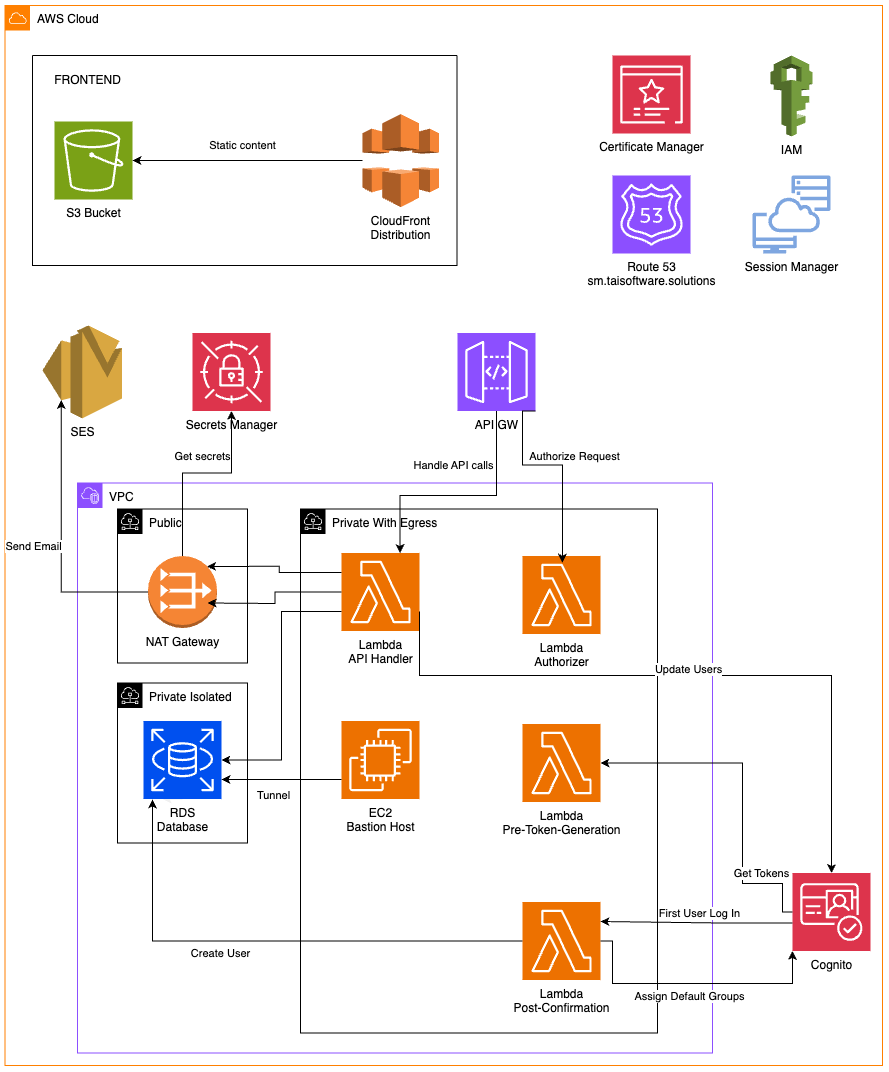
\includegraphics[width=1.1\linewidth]{immagini/infra/full_Infrastructure_services.png}%
    }
    \caption{Architettura del sistema}
    \label{infra_full}
\end{figure}

\FloatBarrier




\section{Configurazione di Rete}

La rete privata è implementata attraverso una \texttt{VPC} (Virtual Private Cloud) all’interno del cloud AWS, segmentata in tre Subnet:

\begin{itemize}
    \item \texttt{Privata Isolata}: per ospitare l’istanza del database.
    \item \texttt{Privata con Egress}: per i servizi che hanno bisogno di accesso a internet, come le Lambda e il Bastion Host.
    \item \texttt{Pubblica}: contiene solo il NAT Gateway per permettere alle risorse nella Subnet Privata con Egress di raggiungere internet senza esporre gli ip pubblici.
\end{itemize}

Per garantire \texttt{disponibilità e resilienza}, ogni categoria di subnet è replicata per le 2 zone di disponibilità della regione AWS Francoforte (eu-central-1):
\begin{itemize}
    \item \texttt{Zona A}: eu-central-1a
    \item \texttt{Zona B}: eu-central-1b
\end{itemize}
\section{Frontend}

Per interagire con il sistema, gli utenti utilizzano una WebApp sviluppata interamente dal mio collega di tirocinio. Il mio contributo è stato principalmente fornire l'infrastruttura necessaria per il deployment dell'applicazione. 
Come anticipato nella sezione

Di seguito è riportato un diagramma che illustra i principali servizi e utenti che interagiscono con questa parte del sistema:

\begin{figure}[ht]  
    \centering
    \makebox[\textwidth][c]{%
        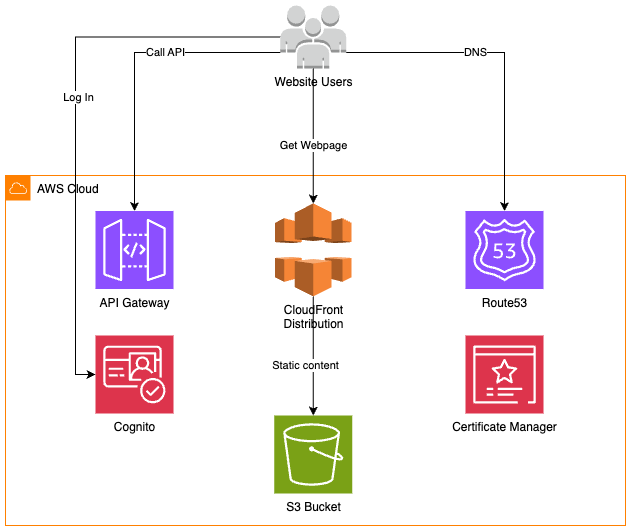
\includegraphics[width=0.8\linewidth]{immagini/infra/frontend.png}%
    }
    \caption{Architettura frontend nel tettaglio}
    \label{imm:infra_frontend}
\end{figure}

\FloatBarrier

-- qui manca da qualche parte il riferimento al "contratto" fatto con la specifica openapi, e che nel mentre dello sviluppo abbiamo aggiunto funzionalita rilevate necessarie

La WebApp è stata sviluppata utilizzando React, il che significa che è stata implementata come una single-page application (SPA). Una SPA è caratterizzata dal fatto che, per ottenere l'intera applicazione, è sufficiente ricevere i file statici iniziali, i quali includono il routing interno e le chiamate alle API per popolare le interfacce utente. Questo approccio elimina la necessità di un server per elaborare dinamicamente le pagine in base alle richieste degli utenti, poiché tale elaborazione avviene sul lato client.

Inizialmente, si era considerato l'utilizzo di \texttt{Next.js}, un framework fullstack per creare applicazioni web che sfrutta React come libreria client. Questo framework avrebbe offerto la possibilità di caricare le pagine ibridamente, sia lato server che lato client, garantendo una maggiore flessibilità. Tuttavia, questa soluzione non era in linea con i requisiti serverless del progetto di tirocinio. Inoltre, l'adozione di Next.js avrebbe comportato un aumento della complessità del sistema, introducendo la necessità di gestire un server aggiuntivo. Considerando che le funzionalità del servizio non richiedevano un approccio così avanzato, l'utilizzo di Next.js non sembrava giustificato.

\vspace{0,3cm}

La \texttt{distribuzione} della WebApp è stata fatta tramite \texttt{CloudFront}, un Content Delivery Network (CDN) progettato per distribuire in modo efficiente contenuti statici su scala globale.
La nostra Web App utilizza un Bucket \texttt{S3} (Simple Storage Service) per immagazzinare la build del frontend. CloudFront agisce come uno strato di distribuzione globale che si interpone tra l'utente finale e il Bucket S3. 

-- qui manca la valutazione di amplify


Per quanto riguarda l'autenticazione con il sistema dalla WebApp, rimando alla sezione \ref{autenticazione}.
\section{Database}

QUI manca la parte dove faccio differenza con DynamoDB


\subsection{Bastion Host}

Il bastion host è una macchina virtuale EC2 che funge da punto di accesso controllato per interazioni di basso livello con l’istanza RDS, come creazione di utenti con privilegi limitati per gli altri servizi e creazione di database e tabelle.  Risiede nella Subnet Privata con Egress per potersi collegare dall’esterno.

\vspace{0,3cm}

L'istanza della macchina EC2 è di classe T2 e size Micro, l'istanza più piccola possibile, con versione Linux AmazonLinux2023.

La risorsa viene inizializzata attraverso scripts \texttt{cloud-init} (per approfondire visitare la \href{https://docs.aws.amazon.com/AWSEC2/latest/UserGuide/user-data.html}{documentazione AWS}) per:

\begin{itemize}
    \item  configurazione iniziale, per installare le dipendenze necessarie, come aws-cli. 
    \item fornire scripts utili tipo get-aws-secrets e db-connect
    \item inizializzare crono di auto-shutdown
\end{itemize}

La gestione delle credenziali di accesso alla macchina è eliminata grazie all’autenticazione tramite SSO, che rimuove inoltre la necessità di esporre il server alla rete pubblica aumentando la sicurezza.

Il bastion è progettato per essere una risorsa temporanea, quindi per ottimizzare efficienza e costi si spegnerà automaticamente dopo 30 minuti di inattività.


\subsection{Database}

Per la gestione dei dati, è stata adottata un'istanza RDS, con configurazione: 
\begin{itemize}
    \item \texttt{engine:} PostgreSQL v16.
    \item \texttt{memoria:} 20GB con la possibiltà di scalare automaticamente fino a 105GB. Memoria SSD di tipo \href{https://docs.aws.amazon.com/AmazonRDS/latest/UserGuide/CHAP_Storage.html#Concepts.Storage.GeneralSSD}{GP2}.
    \item \texttt{istanza:} classe T2 e size Micro.
\end{itemize}
L’istanza viene dispiegata nella subnet privata in modalità Multi-AZ, quindi replicata nelle 2 availability zones, per assicurare alta disponibilità. Nel caso di necessità di scalabilità può essere valutata una migrazione a RDS con Aurora Serverless V2.

Per testare durante lo sviluppo, invece di mantenere tunnel tramite bastion (sezione \ref{sub:connessione_db}) e lavorare sul database dell'ambiente di DEV, ho preferito lanciare un istanza Postgres in locale.

\subsubsection{Gestione utenti}
Il database ha un account amministratore, dedicato alle operazioni di manutenzione attraverso il bastion host. L’unico altro utente è assegnato all’API, con privilegi di R/W sulle tabelle. 
Alla creazione dell’istanza, vengono creati anche i segreti contenenti le credenziali per i suddetti utenti, che verranno consumate tramite Secrets Manager.
Di seguito il codice SQL eseguito per creare l'utente applicativo:

\lstinputlisting[
    language=SQL,
    caption={Creazione utente per l'API con R/W sulle tabelle },
    label={lst:db_utente}
]{code/database/create_db_user.sql}

Questa procedura è stata eseguita manualmente successivamente alla creazione del database, acquisendo la password attraverso Secrets Manager. Inoltre, se vengono create delle tabelle, è necessario assegnare anche i relativi permessi, seguendo le istruzioni dalla riga 4 alla riga 14. 

\subsubsection{Connessione all'istanza}
\label{sub:connessione_db}
Per accedere all'istanza del database, utilizzo il bastion host come tunnel verso l'istanza del database nella rete privata. Questo processo permette di mappare l'indirizzo IP e la porta del bastion (che a sua volta si connette all'indirizzo IP e alla porta privata dell'istanza) in locale. A questo scopo, ho sviluppato uno script bash che automatizza il processo di configurazione e avvio del tunnel. Lo script cerca l'istanza EC2 nell'account AWS e ne estrae l'ID e se la macchina è spenta viene svegliata. Successivamente, recupera le credenziali di accesso al database da AWS Secrets Manager e, infine, avvia una sessione con AWS Systems Manager (SSM) utilizzando come target il bastion.

Ecco il codice bash che implementa questo processo:

\lstinputlisting[
    language=Bash,
    caption={Script bash tunnel.sh per connettersi all'istanza del databse},
    label={lst:tunnel}
]{code/database/tunnel.sh}

Per quanto riguarda AWS SSM, è un servizio che consente di eseguire comandi su istanze EC2 in modo sicuro e senza dover effettuare una connessione diretta tramite SSH. Utilizzando SSM, è possibile gestire le risorse EC2 in modo centralizzato, senza dover esporre le istanze direttamente alla rete pubblica. Utilizzando il comando start-session di AWS SSM, è possibile avviare una sessione interattiva con un'istanza EC2 tramite il bastion host, consentendo l'accesso sicuro al database tramite il tunnel stabilito.

\vspace{0,3cm}

Una volta avviato il tunnel, è possibile collegarsi sostanzialmente in 2 modi:
\begin{itemize}
    \item \texttt{Linea di comando:} con un tool come \texttt{psql} posso avviare una sessione interattiva da terminale.
    
    \lstinline[language=Bash]{psql -p 5432 -h 127.0.0.1 -U username -d database_name}

    \item \texttt{Applicativo:} una applicazione desktop con GUI come \texttt{PGAdmin}, che fornisce molte funzioni per visualizzare e interagire con il database.
\end{itemize}


\subsubsection{Gestione schema e Migrazioni}
Per l'evoluzione dello schema del database, è stato scelto \texttt{Prisma}, che fornisce una solida piattaforma per la gestione delle migrazioni dei dati. Grazie a Prisma, è possibile eseguire in modo efficiente l'aggiornamento dello schema del database, garantendo una transizione fluida e sicura tra le diverse versioni.
Le funzionalità di migrazione offerte da Prisma consentono di apportare modifiche agli schemi del database in modo controllato e reversibile, assicurando la coerenza e l'integrità dei dati durante il processo di evoluzione. L'approccio dichiarativo di Prisma facilita la definizione chiara e concisa delle modifiche da apportare, semplificando così la gestione delle versioni e agevolando il mantenimento della base dati nel corso del tempo. Prisma utilizza il linguaggio proprietario con estenzione .prisma per definire  la struttura delle tabelle, le relazioni tra di esse, i tipi di dati e le regole di validazione.

\vspace{0,3cm}

Per utilizzare Prisma nel progetto, ho scaricato tramite NPM come dipendenza di sviluppo il pacchetto \texttt{prisma}, il tool da linea di comando.

Il file principale contenente lo schema è schema.prisma. Dato che avevo già definito lo schema tramite SQL, mi è bastato eseguire \lstinline[language=Bash]{npx prisma db pull} per inizializzare il file con lo schema del database, da cui sono partito per le successive modifiche.

\vspace{0,3cm}

Ecco il codice con la configurazione iniziale e la definizione della tabella certificati:

\lstinputlisting[
    language=Prisma,
    caption={Definizione dello schema del database in Prisma},
    label={lst:schema_prisma}
]{code/database/schema.prisma}


La keyword \texttt{model} è usata per definire le tabelle con le specifiche di ogni campo.
In \texttt{datasource} definisco il provider, nel mio caso postgresql e l'url di connessione al database, che passo tramite variabile di ambiente.
La keyword \texttt{generator} indica cosa deve essere generato al cambiamento dello schema, al lancio del comando \lstinline[language=Bash]{npx prisma generate}. Sono definiti 2 generatori: client per prisma-client e kysely (quest'ultimo discusso nella sezione \ref{Kysely}).  

\vspace{0,3cm}

\label{prisma_client}
Inoltre, con lo schema Prisma è possibile generare un client da utilizzare nel codice, con la libreria \texttt{prisma-client}. Questo client, chiamato ORM (Object Relational Mapping), offre strumenti per interagire con il database in modo type-safe e astratto tramite un oggetto, eliminando la necessità di scrivere codice SQL manualmente. Tuttavia, offre anche la flessibilità di eseguire query SQL personalizzate se necessario.

Tramite la libreria \texttt{prisma-client}, scaricata come dipendenza di sviluppo e non inclusa nella produzione, vengono eseguite principalmente operazioni di seeding attraverso il comando \lstinline[language=Bash]{npx prisma db seed}. Questo comando esegue il codice definito nel file `seed.ts` situato nella cartella `prisma`, utilizzando il client Prisma per interagire con il database. Prima di utilizzare il client Prisma, è necessario eseguire la generazione per sincronizzare l'ORM con lo schema definito. Di seguito è riportato un esempio di seeding che aggiunge un record nella tabella dei Certificati:

\lstinputlisting[
    language=TypeScript,
    caption={Esempio di seeding},
    label={lst:seeding}
]{code/database/seed.ts}

Da questo esempio possiamo vedere come viene astratta l'interazione con le tabelle del database attraverso l'ORM, chiamando direttamente la creazione sull'oggetto certificati.

\vspace{0,3cm}

Per mantenere l'evoluzione dello schema del database allineata con le modifiche apportate allo schema Prisma, eseguo una migrazione sul database locale utilizzando il comando \lstinline[language=Bash]{npx prisma migrate dev --name v1.x.x}. Questo comando genera un file di migrazione nella directory "migration" sotto "prisma", il quale contiene i comandi SQL necessari per adeguare lo schema del database alle modifiche apportate allo schema.prisma rispetto alla migrazione precedente. È importante sottolineare che questi file di migrazione rappresentano semplicemente una serie di istruzioni SQL che vengono eseguite per aggiornare lo schema del database.

Una volta generato il file di migrazione, procedo con il tunneling verso il database remoto e sostituisco l'URL di connessione nell'ambiente con le credenziali aggiornate. Successivamente, applico la migrazione remota utilizzando il comando \lstinline[language=Bash]{npx prisma migrate deploy}. Quest'ultimo passaggio è fondamentale per sincronizzare le migrazioni con il database remoto, assicurandoci che tutte le modifiche apportate allo schema siano effettivamente applicate.

Il processo che segue la creazione della migrazione locale può essere automatizzato all'interno di un pipeline, il quale esegue automaticamente il comando finale senza richiedere l'avvio manuale del tunnel o il recupero delle credenziali da parte dello sviluppatore. Tuttavia, questa problematica è discussa più approfonditamente nella sezione \ref{evoluzione_db_problematica}.

\section{API}

L’ API è il servizio con cui il Front End comunica per interagire con il Backend, fornendo operazioni di alto livello per le funzioni svolte dal sito web. Adottando un approccio spec-first nella progettazione dell'API, come descritto nella Sezione \ref{openapi_spec}, sono stato in grado di implementare rapidamente gli endpoints, avendo già sviluppato una versione significativa della specifica OpenApi. Questo approccio mi ha fornito tutte le informazioni necessarie in anticipo, riducendo al minimo la necessità di consultare il collega responsabile del Frontend per chiarire eventuali dubbi durante l'implementazione.

Il servizio è distribuito con AWS \texttt{Lambda}, quindi secondo il modello serverless, esposto utilizzando \texttt{APIGateway}.

\vspace{0,3cm}

La REST API è implementata con una singola Lambda, con configurazione: 
\begin{itemize}
    \item \texttt{runtime} NodeJS-20.
    \item \texttt{timeout} 5 secondi.
    \item \texttt{subnet} private with egress per accedere a SecretsManager, SES, Cognito e altri servizi fuori dalla VPC.
    \item \texttt{memoria} 128MB di RAM.
\end{itemize}

L'API Gateway è configurato per inoltrare ogni richiesta, sotto forma di eventi, alla Lambda REST API e per restituire la risposta ritornata da quest'ultima. 
Per consentire l'accesso al servizio da parte di client esterni, che utilizzano Browser Web per utilizzare il sistema, è stato configurato il CORS \cite{rfc6454}, in base all'ambiente:
\begin{itemize}
    \item \texttt{PROD:} l'accesso in produzione è limitato all'URL del frontend, garantendo la sicurezza del servizio.
    \item \texttt{DEV: } in fase di sviluppo, l'accesso è aperto a tutti per facilitare i test e la messa a punto.
\end{itemize}

\vspace{0,3cm}

È stato associato un nome di dominio e un certificato TLS per rendere il servizio accessibile tramite HTTPS attraverso il nome di dominio "api.taisoftware.solutions" (approfondimenti nella sezione \ref{sec:esposizione_dei_servizi}).


\subsubsection{Vantaggi AWS Lambda + API GW}

\begin{itemize}
    \item \texttt{Scalabilità:} AWS Lambda consente di gestire automaticamente la scalabilità delle funzioni in risposta alla domanda. Questo significa che le risorse vengono allocate solo quando necessario, ottimizzando l'utilizzo e riducendo i costi operativi.
    \item \texttt{Gestione semplificata:} La gestione delle risorse, la manutenzione e l'aggiornamento dell'infrastruttura sono affidati a AWS, eliminando la manutenzione e configurazione del server. Ciò consente al team di concentrarsi maggiormente sullo sviluppo delle funzionalità dell'applicazione.
    \item \texttt{Integrazione:} l’integrazione diretta tra AWS Lambda e AWS API Gateway semplifica l’esposizione dell’API e la gestione delle richieste HTTP. API Gateway è configurato per gestire autenticazione, autorizzazione e limitazione del traffico, contribuendo alla sicurezza e stabilità del sistema.
\end{itemize}

\subsubsection{Svantaggi della soluzione}
\begin{itemize}
    \item \texttt{Cold Starts:} Se nessuna Lambda è attiva, il tempo necessario per l'avvio di una nuova istanza di Lambda (chiamato "cold start") può introdurre una latenza iniziale nelle risposte alle richieste.
    \item \texttt{Limiti:} AWS Lambda ha un limite massimo di tempo di esecuzione e ogni istanza ha memoria e CPU fissata.
\end{itemize}

L’API non dovrà fare operazioni di lunga durata e non necessita di tanta memoria, quindi lo svantaggio riguardo ai limiti è trascurabile. Riguardo alle cold starts, se l’API non viene chiamata per un determinato periodo, l’utente che chiamerà il servizio subirà una cold start di qualche secondo, riducendo l’esperienza utente. Se diventasse un problema, si potrebbe valutare di tenere sempre una Lambda “warm” per eliminare le cold start, ma gravando sui costi. Le possibili soluzioni a questa problematica sono discusse nella sezione \ref{lambda_cold_start}.


\subsection{Implementazione}
Per creare una REST API su Lambda in TypeScript, esistono diverse opzioni di framework, come \href{https://www.serverless.com/framework/docs-providers-aws-events-apigateway}{Serverless Framework}. Tuttavia, in azienda mi è stato presentato un mini-framework sviluppato internamente da un membro del team, chiamato \texttt{Micro}. Questo framework si è dimostrato la scelta ideale poiché segue il paradigma "spec first": partendo da una specifica OpenAPI, il framework fornisce uno script di generazione automatica dell'impalcatura (scaffolding) del codice. 
Nella fase di scaffolding, vengono generati:
\begin{itemize}
    \item \texttt{classi} relative ai modelli defiti
    \item \texttt{file} per ogni percorso con firma della funzione e import necessari
    \item \texttt{schema percorsi} in JSON con i dettagli di ogni percorso per la validazione
\end{itemize}


Inoltre, l'attributo operationId, inserito in ogni definizione di percorso, ha garantito un nome univoco per ciascuno di essi, necessario per il naming dei file automaticamente generati.

Micro è configurato per abilitare la \texttt{dependency injection}, un pattern per il quale posso definire servizi, richiedibili dagli altri semplicemente specificandoli nel costruttore. Il motore della dependency injection si occupa di fornire i servizi e di gestire le istanze, ad esempio permettendo di definire un servizio come singleton e gestendone l'utilizzo tra i vari richiedenti. Questo pattern è stato implementato con la libreria \href{https://inversify.io/}{Inversify}, anche se non entreremo nei dettagli. È fondamentale sottolineare questo aspetto, poiché presenteremo in seguito i principali servizi che collaborano per rispondere a una chiamata.

Infine, è importante menzionare che il framework gestisce anche la \texttt{validazione delle richieste}. Ogni richiesta viene confrontata con lo schema dei percorsi, verificando i tipi e i campi richiesti. Questa funzionalità è stata sviluppata durante il tirocinio e ho contribuito al debugging delle varie parti, assicurandomi che il processo di validazione fosse accurato e affidabile. Grazie a questa funzionalità, sono stato in grado di eliminare la maggior parte dei controlli durante lo sviluppo dei percorsi, poiché potevo assumere che i dati fossero corretti.

-- aggiungere cdk compatibility

\subsubsection{Kysely - query builder}
\label{Kysely}

\vspace{0,3cm}

La decisione di escludere Prisma Client (sezione \ref{prisma_client}) dalla produzione è stata motivata dalla sua eccessiva pesantezza e dalle dimensioni del runtime che avvia in background. Questo comporta un aumento sia della memoria RAM utilizzata che delle dimensioni del bundle di esecuzione, raddoppiando il volume dei moduli da 100 MB a 200 MB. 

Questi fattori diventano problematici soprattutto in ambienti serverless, poiché aumentano il tempo di caricamento iniziale e il consumo di memoria di base. Inoltre, la configurazione di Prisma Client con AWS Lambda, come descritto nella \href{https://www.prisma.io/docs/orm/prisma-client/deployment/serverless/deploy-to-aws-lambda}{documentazione di Prisma}, consiglia l'utilizzo di framework come \texttt{SST} o \texttt{SAM}, che non sono stati scelti per questo progetto. Di conseguenza, avrei dovuto affrontare una configurazione più complessa e laboriosa.

\vspace{0,3cm}

In alternativa, per la creazione di query dall'API,ho scelto di utilizzare la libreria \texttt{Kysely}, un query builder che offre vantaggi simili a Prisma Client ma con una minore complessità e leggerezza. A differenza di Prisma, Kysely non richiede un runtime, ma trasforma direttamente il codice in query SQL e si occupa della formattazione e dell'esecuzione di prepared statements per prevenire le injection SQL. 

Per utilizzare Kysely, è necessario definire un'interfaccia contenente lo schema del database. In questo contesto, ho utilizzato la libreria \texttt{prisma-kysely}, che permette di generare automaticamente l'interfaccia a partire dalla definizione dello schema in Prisma (configurazione del generatore nel listing \ref{lst:schema_prisma}). Questo approccio consente di definire lo schema una sola volta in Prisma e di generare automaticamente l'interfaccia necessaria per Kysely, semplificando così il processo di sviluppo e manutenzione del codice.


\subsubsection{Autorizzazione a grana fine}
\label{context_service}
Nel context dell'evento, come descritto nella sezione \ref{authorizer}, vengono trasmessi i gruppi di appartenenza dell'utente e l'ID dell'utente nel database. Queste informazioni sono essenziali per eseguire autorizzazioni specifiche basate sull'utente e sull'operazione richiesta. Ad esempio, l'ID dell'utente può essere considerato come l'identificatore del chiamante e può essere utilizzato per limitare l'accesso solo alle risorse associate a quell'utente.

Per semplificare il processo di autorizzazione, ho sviluppato un servizio dedicato, \texttt{context service}: 

\lstinputlisting[
    language=TypeScript,
    caption={Servizio per gestire l'autorizzazione degli utenti},
    label={lst:auth_service}
]{code/api/context_service.ts}

Non sono stati inclusi dettagli implementativi relativi al testing locale, come la sostituzione dei gruppi e dell'ID estratti dal contesto con valori costanti, per mantenere la brevità del codice. Gli import sono stati omessi dall'inizio del file per lo stesso motivo.

\label{context_service_funzioni}
Le funzioni \texttt{getGroups} e \texttt{getCallerUserId} sono incaricate di estrarre i dettagli rilevanti dal contesto dell'evento. 

Successivamente, la funzione \texttt{authorizeUserOrThrow} viene utilizzata per gestire l'autenticazione dell'utente in base ai ruoli richiesti in un percorso specifico e per restituire un errore 403 Forbidden in caso di autorizzazione negata. Questa funzione richiede come parametri i ruoli accettati per il percorso e, opzionalmente, l' ID da verificare se l'utente appartiene a un determinato gruppo. 

È importante notare che la funzione ritorna il gruppo a cui l'utente appartiene, consentendo controlli successivi se necessario. Tuttavia, è fondamentale tenere presente che questo servizio presenta alcune limitazioni. Ad esempio, è essenziale che i gruppi vengano passati in ordine di autorità per 2 principali motivi:
\begin{itemize}
    \item La funzione restituirà il primo gruppo trovato, quindi è importante che il ruolo con maggiori autorizzazioni sia posizionato all'inizio della lista per garantire i privilegi appropriati.
    \item È necessario effettuare controlli sull'ID dell'utente solo se non possiede un ruolo con privilegi maggiori.
\end{itemize}

Infatti, il ruolo admin è posizionato di default all'inizio della lista dei gruppi.

Per un esempio pratico di utilizzo di questo servizio, si rimanda alla sezione \ref{esempio-endpoint}.

\subsubsection{Accesso al Database}
\label{db_service}
Per facilitare l'accesso al database, ho sviluppato un servizio dedicato alla gestione della connessione, il quale si adatta sia all'ambiente locale che a quello di produzione. In ambiente locale, vengono utilizzate credenziali "hard coded" relative a un'istanza locale, mentre in produzione le credenziali del database vengono recuperate tramite AWS Secrets Manager. Le credenziali vengono ottenute all'inizializzazione della Lambda e tenute in memoria per non effettuare una chiamata a Secrets Manager ad ogni richiesta.

Il servizio è configurato come un singleton, il che significa che mantiene una singola istanza della connessione attiva e la riutilizza per ogni chiamata al database, anziché aprirne una nuova ogni volta.

Questo servizio offre due modalità di accesso al database:

\begin{itemize}
    \item \texttt{Pool:} Consente di comunicare tramite una connessione diretta con pg, adatto per operazioni di basso livello e semplici query SQL.
    \item \texttt{Kysely:} Fornisce un'istanza di Kysely, inizializzata con la connessione a pg, ottimizzata per eseguire query in modo efficiente e sfruttando i vantaggi del query builder.
\end{itemize}

In questo modo, gli sviluppatori hanno la flessibilità di scegliere lo strumento più adatto in base alle specifiche esigenze di ogni situazione.

\lstinputlisting[
    language=TypeScript,
    caption={Servizio per accedere al database tramite pg e kysely},
    label={lst:db_service}
]{code/api/db_service.ts}

\subsubsection{Accesso ai dati}
\label{dao}
Per astrarre l'accesso al database e la creazione delle query, ho sviluppato un servizio DAO per ogni risorsa del database. Questo approccio consente di raggruppare la logica e i controlli necessari, riducendo al minimo la duplicazione del codice. Ogni DAO implementa le operazioni CRUD standard, ovvero create, read (getAll e getOne), update e delete, oltre a eventuali funzionalità aggiuntive in base alle esigenze del sistema.

L'implementazione di questi servizi è diventato necessario poiché ho deciso di non utilizzare Prisma Client (sez. \ref{prisma_client}), che avrebbe fornito un'interfaccia simile per l'accesso alle risorse del database.

Nei servizi DAO, la connessione al database è gestita tramite il servizio database service (sezione \ref{db_service}), mentre la costruzione delle query avviene mediante l'utilizzo della libreria Kysely (sezione \ref{Kysely}). 

\vspace{0,3cm}

Di seguito è riportato un esempio del DAO per l'operazione getAll sulla risorsa Utenti, analogo agli altri DAO per le diverse risorse, che utilizza l'istanza di Kysely fornita dal database service per costruire la query. 

\lstinputlisting[
    language=TypeScript,
    caption={Esempio di DAO per gli utenti},
    label={lst:dao_utenti}
]{code/api/getAllUsersDAO.ts}

Questa funzione,  essendo una getAll, implementa la paginazione, il filtraggio e l'ordinamento, come anticipato nella sezione \ref{Paginazione}.
La trasformazione di questi filtri e dell'ordinamento per kysely viene gestita da un servizio chiamato \texttt{QueryFormatter}, del quale non entreremo nei dettagli.


\subsection{Esempio di endpoint}
\label{esempio-endpoint}

Sotto è presentato il codice per gestire la richiesta GET /users, utilizzando il servizio di autorizzazione (sezione \ref{context_service}) e il dao della risorsa utenti (sezione \ref{dao}). Questa implementazione illustra come l'uso del context service e del DAO semplifichi la scrittura dei vari endpoint dell'API, riducendo al minimo la duplicazione del codice e astraendo i vari procedimenti intermedi.

\lstinputlisting[
    language=TypeScript,
    caption={Esempio di Endpoint handler per GET /users},
    label={lst:getUsers_handler}
]{code/api/getAllUsersHandler.ts}

Nella definizione OpenAPI dell'endpoint (riportata nel listing \ref{lst:openapi_getAll}), sono presenti due tags: Users e HumanResources. Come discusso in precedenza nella sezione \ref{Tags}, i tags aggiuntivi rispetto a quello della risorsa definiscono chi può accedervi.. L'autorizzazione del percorso avviene tramite il context service utilizzando la funzione authorizeUserOrThrow, descritta in dettaglio nella sezione \ref{context_service_funzioni}, passando quindi in questo caso il gruppo HR.

Dopo l'autorizzazione, viene utilizzata un'istanza del DAO utenti per chiamare la funzione getAll (definita nel listing \ref{lst:dao_utenti}), passando i parametri di paginazione. 

Infine, la risposta contenente gli utenti e il codice di successo viene restituita all'API Gateway per inoltrarla al chiamante.

% \subsection{Notifiche}

\subsection{Testing}
\label{testing_api}
Durante lo sviluppo servizio, ho adottato due approcci distinti per testare il sistema in diversi contesti: il testing locale e il testing del servizio dispiegato:

\begin{itemize}
    \item \texttt{Testing Locale:} Per testare ogni endpoint, ho sviluppato dei test utilizzando la libreria \href{https://jestjs.io/docs/getting-started}{\texttt{Jest}}, una delle più popolari per il testing delle API, nota per la sua flessibilità e le numerose funzionalità offerte. I test sono organizzati per risorsa e includono gli endpoint CRUD principali, nonché qualsiasi funzionalità aggiuntiva implementata.
    Di seguito è presentato un esempio di test in TypeScript utilizzando Jest per verificare il funzionamento dell'endpoint GET /users:

    \lstinputlisting[
        language=TypeScript,
        caption={Esempio di testing in Jest per GET /users},
        label={lst:test_getAllUsers}
    ]{code/api/testing.ts}

    Le righe 2 e 3 riguardano la generazione di un evento emulato simile a quello che si verificherebbe con l'API Gateway in produzione. Successivamente, dalle righe 4 alla 9, viene eseguita la chiamata alla funzione responsabile del percorso, mentre dalle righe 10 alla 13 vengono effettuati dei controlli per valutare il successo del risultato ottenuto.

    \item \texttt{Testing del Servizio:} Per effettuare il testing della REST API, ho impiegato \href{https://www.postman.com/}{\texttt{Postman}}, un'applicazione desktop dotata di un'interfaccia che consente di creare e organizzare chiamate HTTP. Inoltre, ho sfruttato la funzionalità di autorizzazione nella sezione Oauth 2.0, la quale semplifica il processo di recupero e refresh dell'access token, inserendolo automaticamente nelle richieste. Questo strumento si è rivelato estremamente utile nel rilevare rapidamente eventuali bug durante lo sviluppo, specialmente per le componenti che non potevano essere testate in locale, come l'authorization handler e il preTokenGeneration handler, le quali richiedono un ambiente specifico non replicabile in locale.
\end{itemize}


Nella sezione \ref{testing_pipeline}, si illustra come i test scritti in JEST possano fungere da unit test nella pipeline di rilascio.




\section{Gestione Utenti e Accessi}

Per la gestione delle identità e degli account degli utenti del sistema, è stato scelto \texttt{AWS Cognito}. In particolare, è stata adottata la soluzione \texttt{Cognito User Pools}, che offre un servizio completo per la gestione degli utenti, dell'autenticazione e dell'autorizzazione.

All'interno della user pool sono stati creati dei gruppi, ciascuno associato a uno dei ruoli descritti nella sezione \ref{ruoli}. 
I gruppi creati sono utilizzati per implementare un sistema di \texttt{Role-Based Access Control (RBAC)}, che consente di assegnare ai vari utenti di assumere uno o più di questi gruppi in base ai privilegi e ai permessi necessari per le loro attività.

includere definizione user:id come attributo, discusso dopo a cosa serve

\subsection{Creazione Utenti}

Una volta effettuato l'accesso utilizzando il metodo di login descritto nella prossima sezione, viene automaticamente creato un utente nella User Pool con le informazioni recuperate dall'identity provider.
Per automatizzare la creazione degli utenti nel database, l'aggiunta dei gruppi di default e l'inizializzazione dell'utente nella User Pool di Cognito, è stato individuato un trigger che può essere aggiunto alla user pool stessa. Questo Lambda trigger, noto come \href{https://docs.aws.amazon.com/cognito/latest/developerguide/user-pool-lambda-post-confirmation.html}{\texttt{post-confirmation}}, viene attivato solo al primo login riuscito di ciascun utente. Questa funzione consente di eseguire azioni personalizzate avendo a disposizione come informazioni le generalità dell'utente attraverso l'evento passato da Cognito. Di seguito è riportato il codice della funzione Lambda:

\lstinputlisting[
    language=TypeScript,
    caption={User Pool Post Confirmation Lambda Trigger},
    label={lst:postConfirmation}
]{code/cognito/postConfirmation.ts}

Inizialmente, vengono definiti un array di costanti \texttt{defaultGroups}, che contiene i gruppi di default per gli utenti, e un oggetto \texttt{userToGroupsMap}, indicizzato con le email degli utenti, che consente di associare ad alcuni utenti specifici i gruppi che devono possedere,  (righe 1-2).

La funzione richiede i seguenti servizi nel suo costruttore: \texttt{usersDao} (sez. \ref{dao}) e \texttt{CognitoGroupService}. Quest'ultimo utilizza la AWS SDK per effettuare chiamate all'API di Cognito, ma non entreremo nei dettagli di implementazione.

Essensialmente vengono compiuti i seguenti passi:

\begin{itemize}
    \item \textbf{Estrazione dei dati dell'utente dall'evento:}
    I dati dell'utente vengono estratti dall'evento attraverso la variabile \texttt{event.userName} e \texttt{event.request.userAttributes} (righe 10-12). 

    \item \textbf{Inizializzazione dei dati dell'utente:}
    Inizialmente, i dati dell'utente vengono estratti dall'evento e popolati con i valori corrispondenti (righe 13-20), che vengono quindi memorizzati nella variabile userData. Successivamente, vengono definiti i gruppi dell'utente, recuperandoli dall'oggetto \texttt{userToGroupsMap} se presenti, altrimenti utilizzando i \texttt{defaultGroups} (righe 21-22). Infine, userData viene aggiornato con i gruppi relativi (righe 24-27).
    
    \item \textbf{Assegnazione dell'utente ai gruppi:}
    Utilizzando il servizio \texttt{cognitoGroupsService}, l'utente viene aggiunto ai gruppi definiti in \texttt{userGroups} nella user pool di Cognito (righe 28-29).

    \item \textbf{Creazione dell'utente nel database:}
    Utilizzando il DAO degli utenti, l'utente viene creato nel database con le informazioni ottenute (righe 30-31).

     \item \textbf{Aggiornamento attributi utente nella UserPool:}
    Infine, utilizzando l'ID dell'utente appena creato, procedo con l'aggiornamento dell'attributo personalizzato "custom:user\_id" dell'utente nella user pool, utilizzando il servizio \texttt{CognitoGroupsService} (riga 39).
    
\end{itemize}

\subsection{Autenticazione}

\label{autenticazione}
 - specificare login dalla web app qualche parte
Il sistema Skill Manager è progettato per i dipendenti aziendali di TAI, che utilizzano Gmail come posta elettronica aziendale. Per semplificare il processo di login e sfruttare le credenziali già in loro possesso, è stata scelta la federazione con Google come Identity Provider (IdP) per la user pool di Cognito.

-- qui manca configurazione resource server, scopes, domain names, callback urls

\subsubsection{OauthFlow}
Il processo di login si basa sul framework Oauth 2.0, adottato da Cognito.

Durante la fase di creazione dei token, i gruppi a cui un utente appartiene vengono automaticamente inclusi nell'access token da Cognito sotto il claim \texttt{cognito:groups}, mentre gli attributi dell'utente nella user pool non vengono automaticamente aggiunti ai token. Pertanto, per inserire l'ID dell'utente nell'access token, è stato aggiunto un ulteriore Lambda trigger alla user pool, chiamato \href{https://docs.aws.amazon.com/cognito/latest/developerguide/user-pool-lambda-pre-token-generation.html#user-pool-lambda-pre-token-generation-accesstoken}{pre-token-generation}. Questo trigger viene attivato prima della generazione di ciascun access token e offre la possibilità di aggiungere o sovrascrivere dei custom claims e dei gruppi. La funzione riceve da Cognito le informazioni sull'utente, inclusi i gruppi e gli attributi della User Pool. 

Di seguito è presentato il codice, in cui viene estratto l'ID dell'utente dall'evento e successivamente aggiunto ai claims personalizzati dell'access token.

\lstinputlisting[
    language=TypeScript,
    caption={User Pool Pre Token Generation Trigger},
    label={lst:preTokenGeneration}
]{code/cognito/preTokenGeneration.ts}

Ecco un diagramma di sequenza che illustra il processo di login e le varie risorse coinvolte nel processo.

\begin{figure}[ht]
    \centering
    \makebox[\textwidth][c]{%
        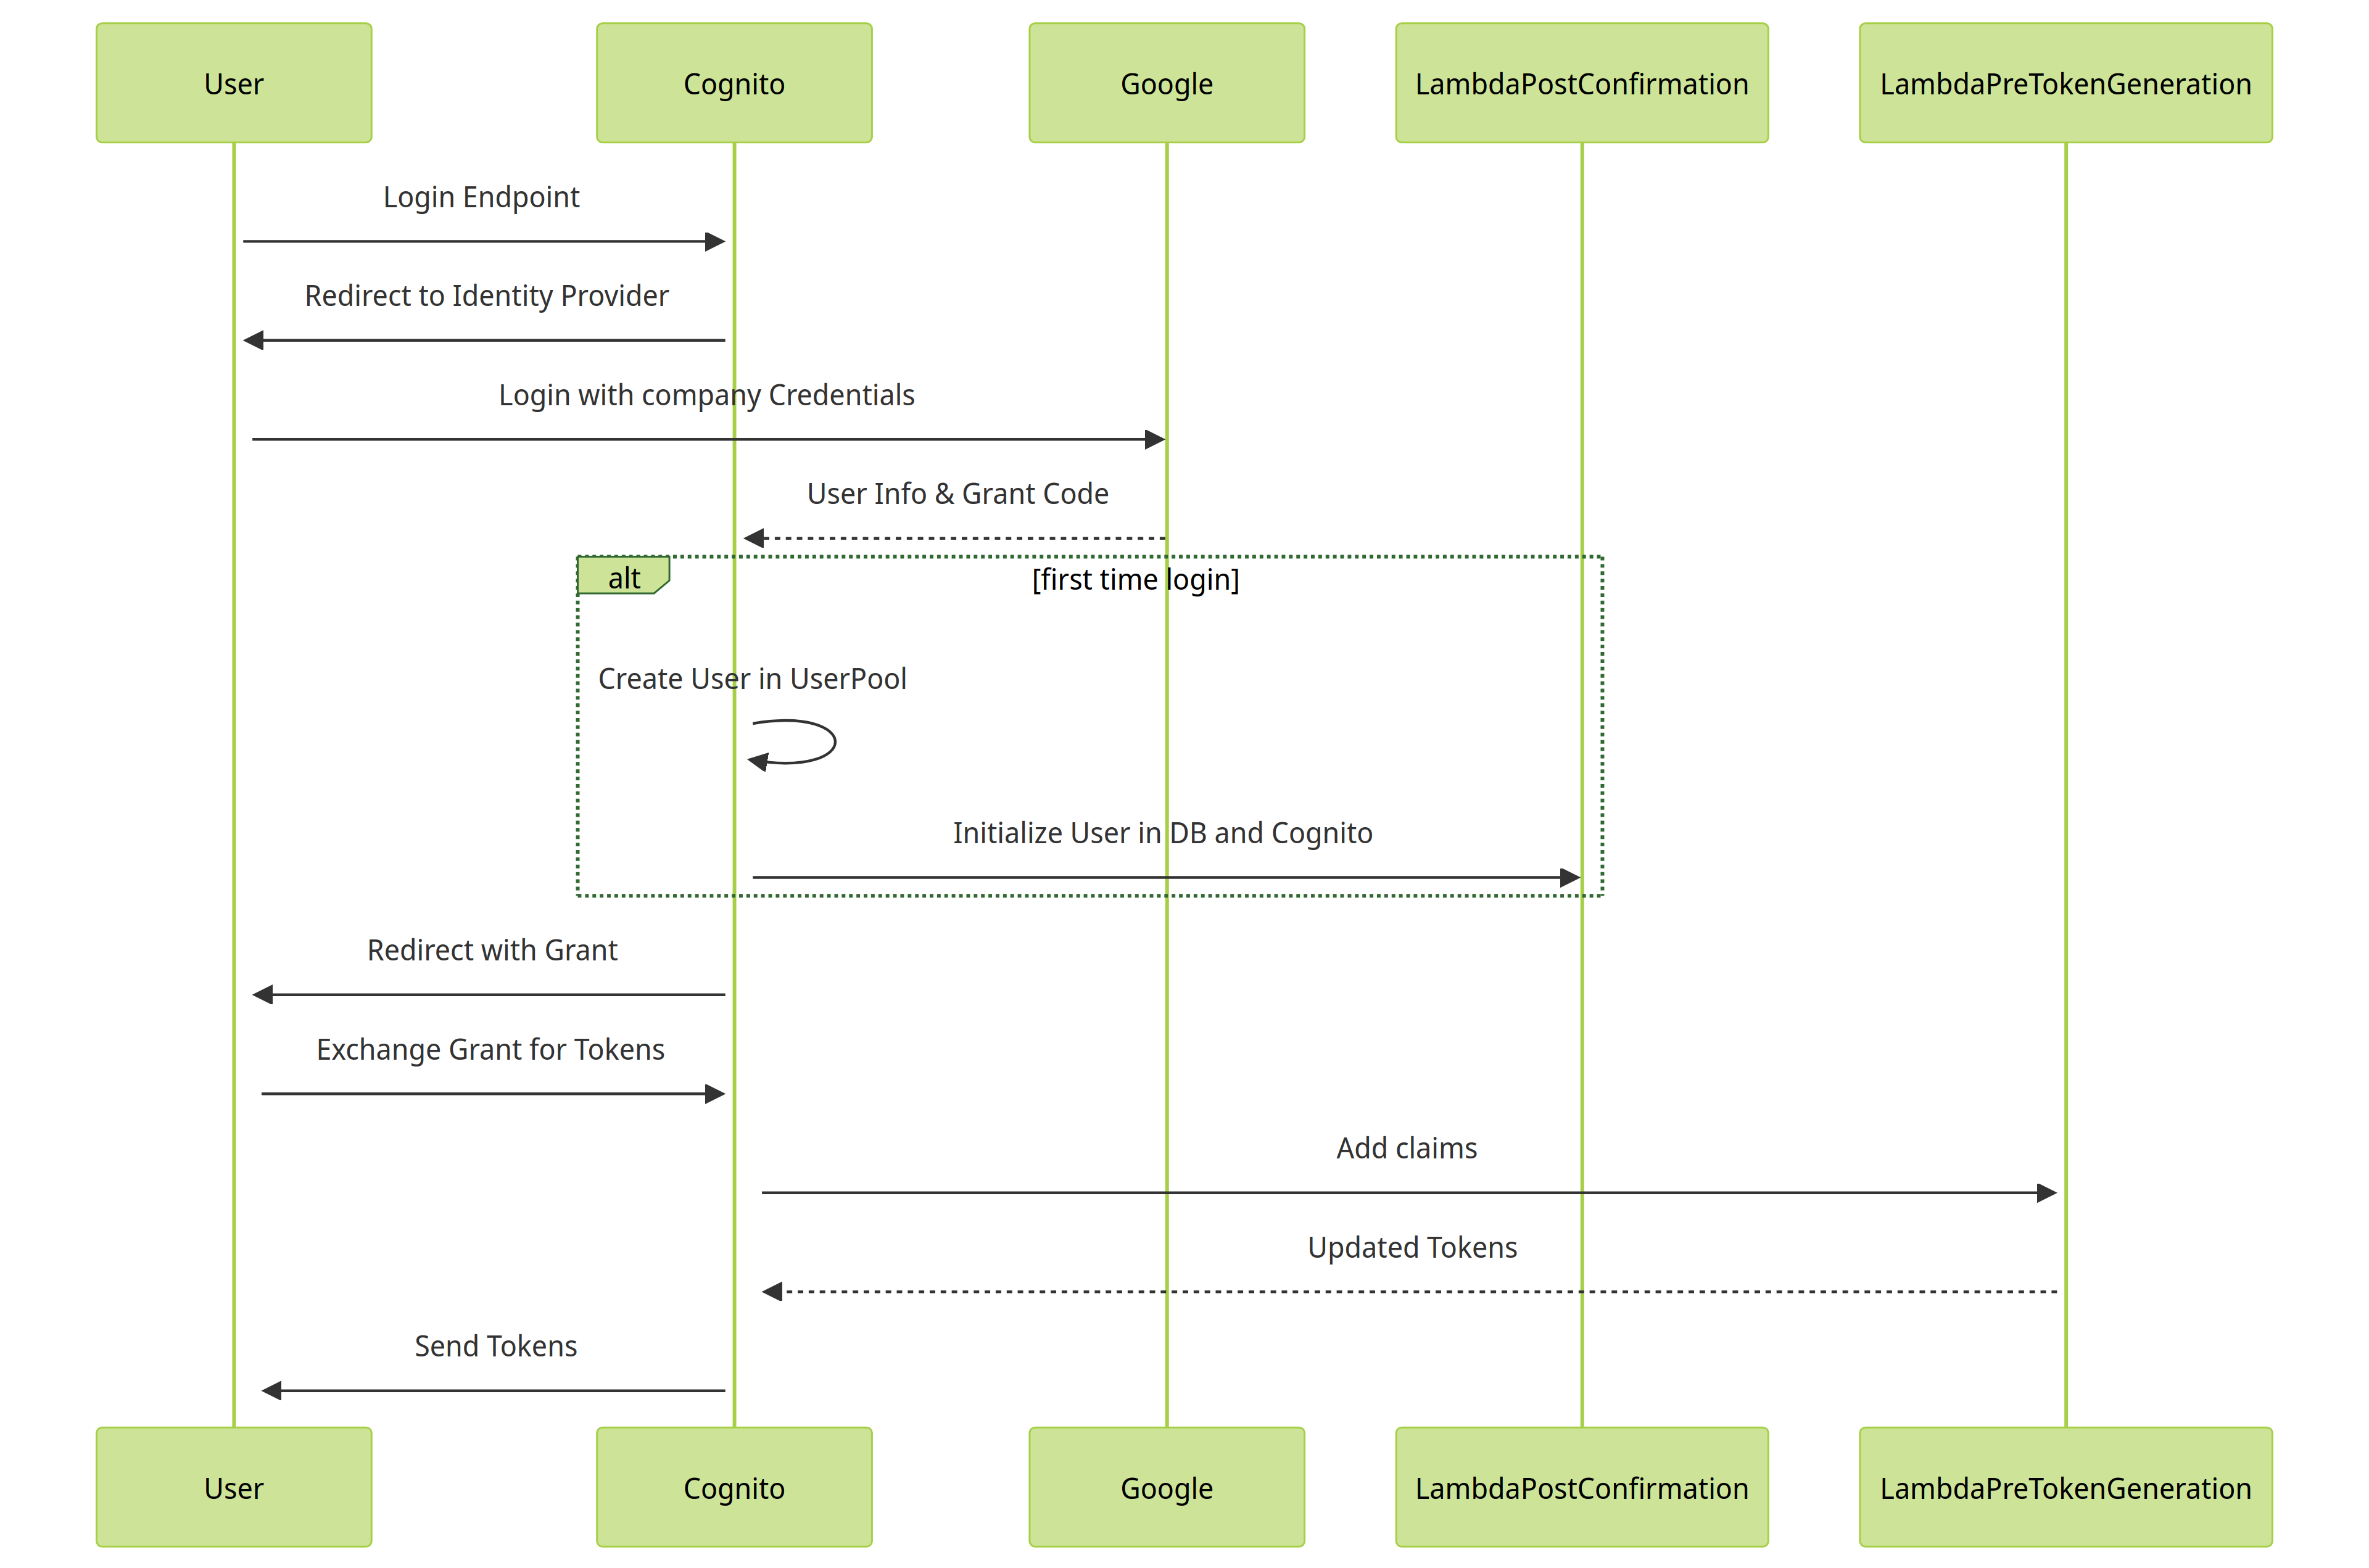
\includegraphics[width=1.1\linewidth]{immagini/oauth_flow.png}%
    }
    \caption{Diagramma di sequenza OauthFlow 2.0}
    \label{auth_sequence}
\end{figure}

\FloatBarrier


\subsection{Autorizzazione}

\label{authorizer}
Dopo aver effettuato l'accesso al sistema e ottenuto un access token (come descritto nella sezione \ref{autenticazione}), l'utente deve includerlo in tutte le richieste alla REST API per garantirne la sicurezza e l'autorizzazione.\
Per fare questo, il client aggiunge un header \texttt{Authorization} nella richiesta HTTP, con il valore \texttt{"Bearer {token}"} \cite{rfc6750}, dove {token} è l'access token ottenuto in fase di autenticazione.

\vspace{0,3cm}
Per gestire la validazione del token, è stato implementato un \texttt{Custom Authorizer} basato su una funzione Lambda. Questa funzione è stata configurata come authorizer nell'integrazione tra la lambda REST API e l'API Gateway, venendo quindi invocata prima di ogni chiamata per autorizzare la richiesta. Solo gli utenti con un token valido possono accedere al servizio. A seconda del risultato della validazione, l'authorizer genera una risposta che contiene le seguenti informazioni:

\begin{itemize}
    \item \textbf{PrincipalId:} L'ID dell'utente nella user pool, se il token è valido.
    \item \textbf{Policy document:} Un documento che specifica le azioni che l'utente è autorizzato a compiere.
    \item \textbf{Effect:} "Allow" se l'utente è autorizzato, "Deny" se non lo è.
    \item \textbf{Context:} Un oggetto opzionale che può contenere informazioni aggiuntive da trasmettere alla funzione successiva.
\end{itemize}
Queste informazioni sono utilizzate dall'API Gateway per determinare se accettare o rifiutare la richiesta del client. Questo processo costituisce il \texttt{primo strato di sicurezza} per il controllo dell'accesso alle risorse del sistema (fase 7 della imm. \ref{auth_cloud}).

Il codice dell'authorizer, che riflette i procedimenti illustrati fino ad ora, può essere consultato nell'Appendice, nella sezione \ref{lst:authorizer-codice}.

\vspace{0,3cm}

Il \texttt{secondo strato di sicurezza} è implementato dalla API, che utilizza le informazioni presenti nel context, quali gruppi e ID utente, per eseguire un'autorizzazione più granulare (fase 9 della imm. \ref{auth_cloud}, vedi dettagli nella sezione \ref{context_service}).
Queste informazioni sono contenute nell'access token, vengono recuperate dall'authorizer in fase di decodifica del token, successivo alla validazione, e poi inserite nel context.

\vspace{0,3cm}

I seguenti diagrammi illustrano l'interazione tra le varie risorse nel processo di autorizzazione di una richiesta. Nel diagramma di sequenza si assume che l'utente sia già in possesso dell'access token e sono rappresentati anche gli errori che possono essere restituiti al client. Nel secondo diagramma si presume che l'autorizzazione sia andata a buon fine.

% valutare se mettere qui la lambda pre token generation - sicuramente andrà nel diagramma dell'autorizzazione
% rivedere naming delle entità

\begin{figure}[ht]
    \centering
    \makebox[\textwidth][c]{%
        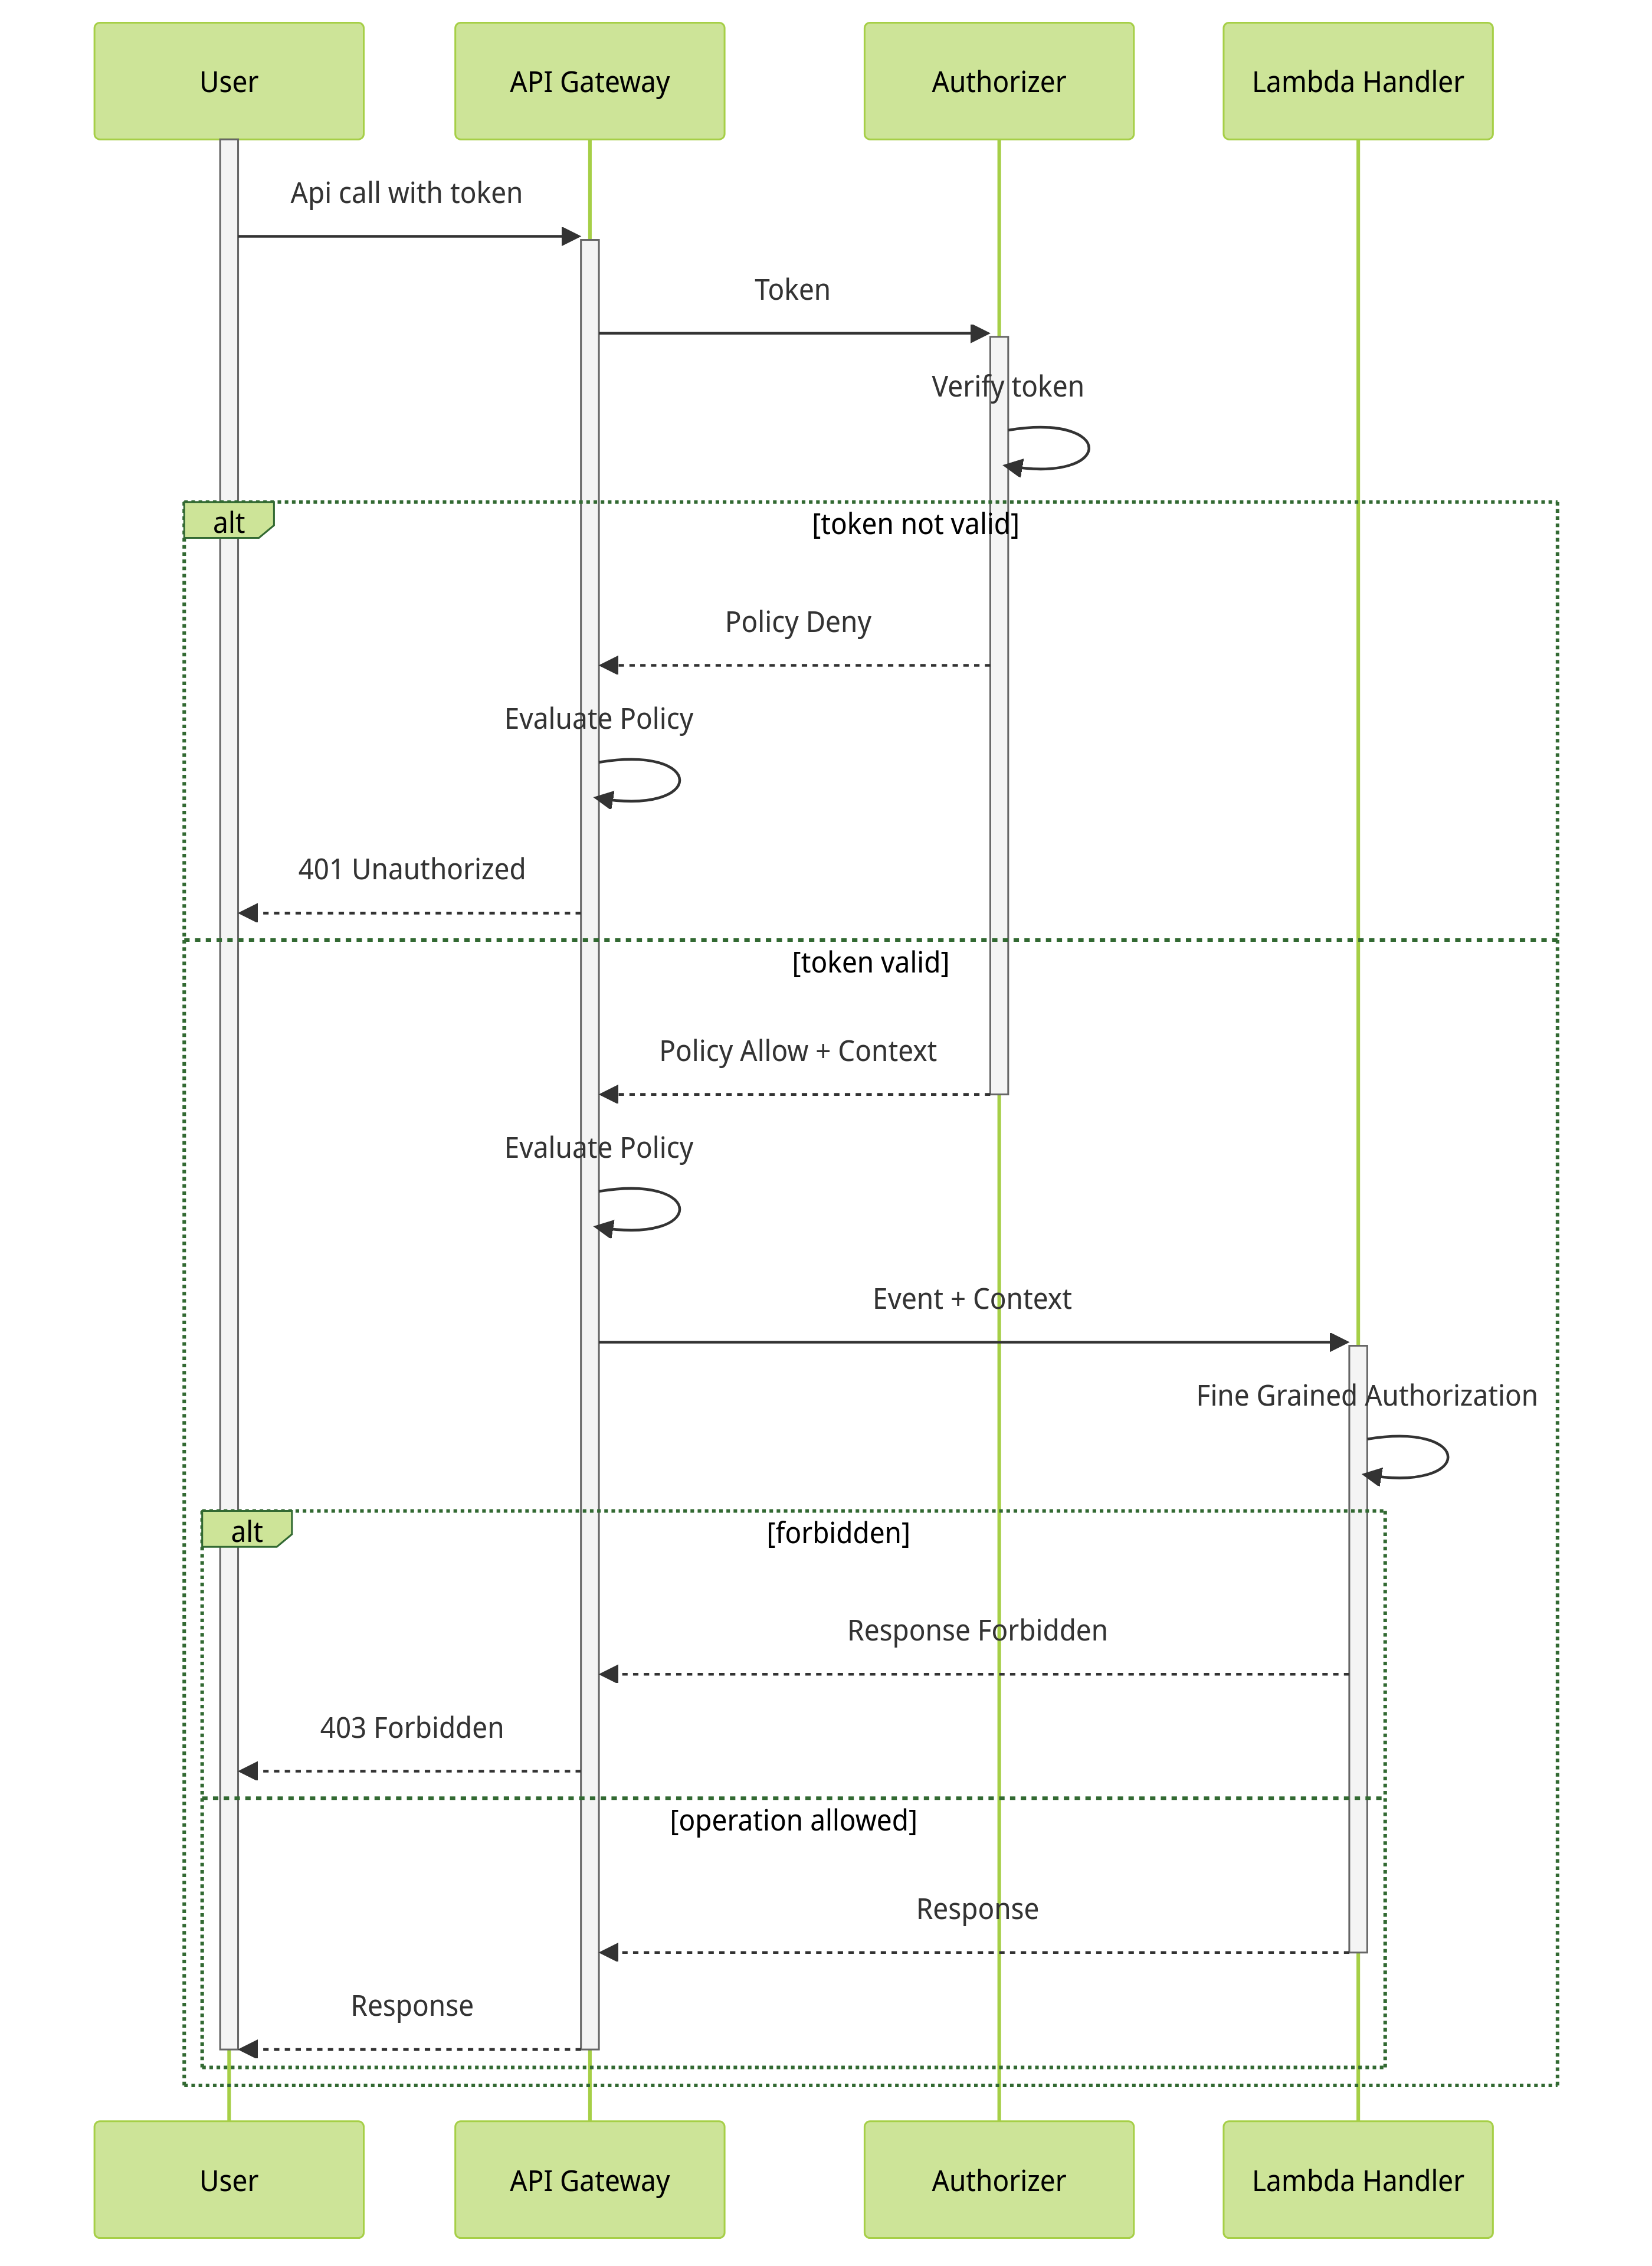
\includegraphics[width=0.9\linewidth]{immagini/Authorization_Flow.png}%
    }
    \caption{Diagramma di sequenza del flusso di autorizzazione}
    \label{auth_sequence}
\end{figure}

\FloatBarrier


\begin{figure}[ht]  
    \centering
    \makebox[\textwidth][c]{%
        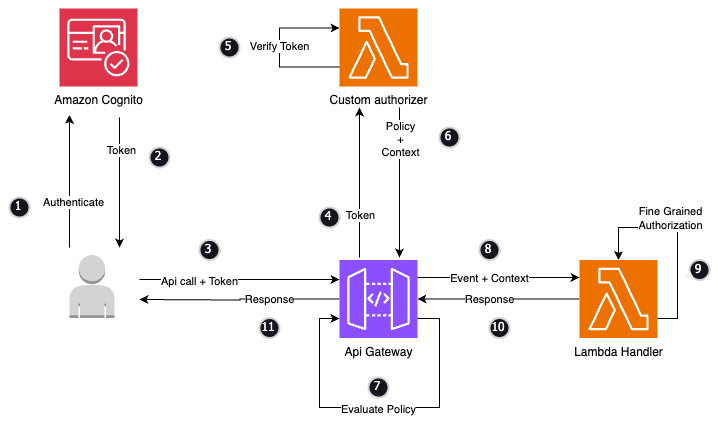
\includegraphics[width=0.9\linewidth]{immagini/AuthFlow_white.png}%
    }
    \caption{Flusso di autorizzazione del sistema andato a buon fine}
    \label{auth_cloud}
\end{figure}

\FloatBarrier


\section{Esposizione dei Servizi}
\label{sec:esposizione_dei_servizi}
Il sistema Skill Manager espone 2 servizi alla rete pubblica, sotto i domini:
\begin{itemize}
    \item \texttt{Web App:}     app.sm.taisoftware.solutions
    \item \texttt{REST API:}		api.sm.taisoftware.solutions
\end{itemize}

Per rendere i servizi accessibili tramite questi nomi di dominio sono stati utilizzati i servizi AWS \texttt{Route53} e \texttt{Certificate Manager}.

\vspace{0.3cm}

\subsection{Certificate Manager}

Nel processo di validazione e creazione dei certificati ACM, è necessario seguire una procedura di proof of ownership del dominio per cui viene richiesto il certificato. Questo processo coinvolge la creazione di record di tipo CNAME sul dominio stesso, come illustrato nella sezione \ref{route53_config}. Questi record consentono ai servizi di ACM di procedere con l'emissione e la validazione del certificato, che sarà firmato dalla certification authority di AWS.

Questo processo è stato formalizzato nell'RFC 8555 \cite{rfc8555} nel 2019, al fine di standardizzare le procedure implementate dai fornitori di servizi cloud.
Nell'introduzione, infatti, è descritto come le entità certificate authority (CA) possano utilizzare procedure basate su DNS per effettuare la proof of ownership dei domini.

Una volta che il certificato ACM è stato prodotto e validato utilizzando la procedura illustrata, poiché le risorse ACM e Route53 sono deployate nello stesso account, il certificato è in grado di auto-rinnovarsi. Successivamente, sarà possibile associare questo certificato a CloudFront e API Gateway per consentire l'esposizione sicura dei servizi tramite HTTPS, utilizzando lo stesso certificato SSL/TLS.

\vspace{0.3cm}
\subsection{Route 53}
\label{route53_config}

Route 53 è stato configurato per permettere la gestione del dominio "sm.taisoftware.solutions". 

Inizialmente, è stata creata una hosted zone dedicata per questo dominio all'interno di Route 53. Quando si crea una hosted zone in Route 53 per un determinato dominio, vengono automaticamente forniti quattro name server (NS) che agiscono come autorità per quel dominio. Questi name server sono quindi utilizzati per rispondere alle richieste DNS relative al dominio stesso. Di conseguenza, la zona pubblica Route53 rappresenta l'autorità per quel dominio.

Per consentire al mio account di gestire il dominio di terzo livello "sm.taisoftware.solutions", è stata effettuata una delega di dominio dal dominio di secondo livello "taisoftware.solutions", che risiede in un account AWS aziendale, tramite la creazione di un record NS nella hosted zone di quel dominio. Questo record NS punta ai 4 name server della hosted zone sul mio account. (, aggiungere altro?)

Questo procedimento è formalizzato nell'RFC 1035 \cite{rfc1035}, il quale stabilisce gli standard per il sistema di nome di dominio (DNS) e la sua implementazione. In particolare, la sezione 3.3.11 di tale documento definisce il formato del campo NS, specificando i dettagli riguardanti la gestione dei name server autoritativi per un dominio.

\vspace{0,3cm}

All'interno della hosted zone, sono stati definiti vari record DNS per indirizzare il traffico verso le risorse appropriate:

\begin{itemize}
    \item Record NS e SOA: Questi record definiscono i name server autorizzati per il dominio e forniscono informazioni sull'autorità del dominio, garantendo una corretta risoluzione dei nomi di dominio.
    \item Record CNAME: È stato configurato un record CNAME per la verifica del certificato TLS emesso per "*.sm.taisoftware.solutions" tramite AWS Certificate Manager (ACM). Questo record permette la verifica della proprietà del dominio durante la procedura di ottenimento del certificato e abilita le connessioni HTTPS.
    \item Record A e AAAA: Questi record consentono di indirizzare il traffico verso le relative risorse, sia tramite IPv4 (record A) che IPv6 (record AAAA).
    \begin{itemize}
        \item "api.sm.taisoftware.solutions" con target l'API Gateway.
        \item "app.sm.taisoftware.solutions" con target la distribuzione CloudFront della Web App.
    \end{itemize}
\end{itemize}
\section{DevOps}
\label{sec:devops}


\begin{figure}[ht]
    \centering
    \makebox[\textwidth][c]{%
        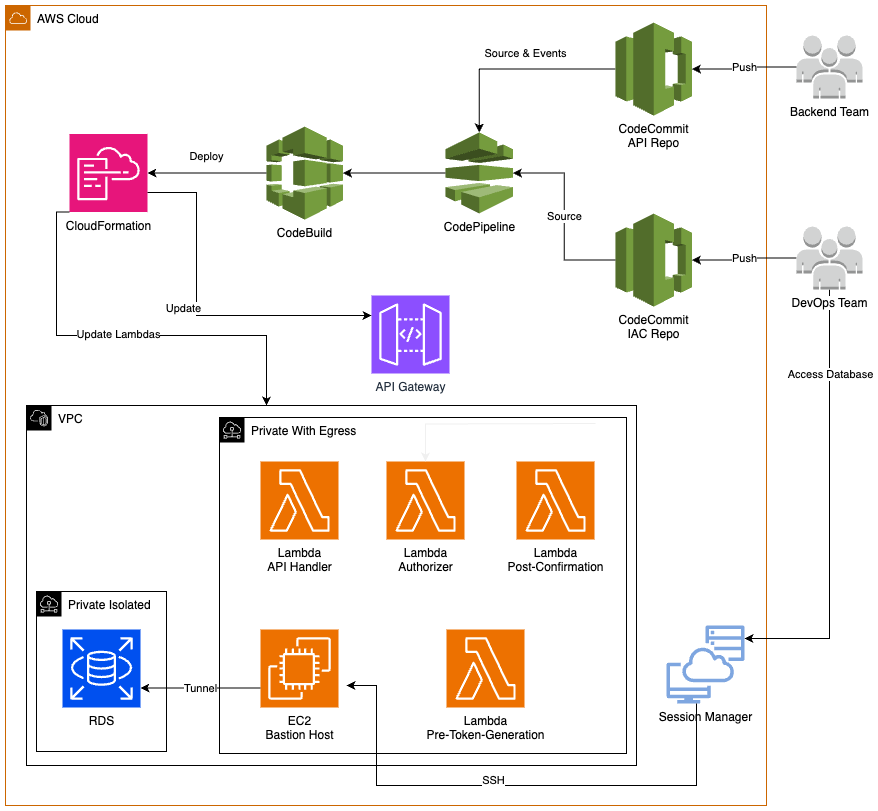
\includegraphics[width=0.9\linewidth]{immagini/infra/backend_devops.png}%
    }
    \caption{Diagramma DevOps Backend}
    \label{auth_sequence}
\end{figure}


\begin{figure}[ht]
    \centering
    \makebox[\textwidth][c]{%
        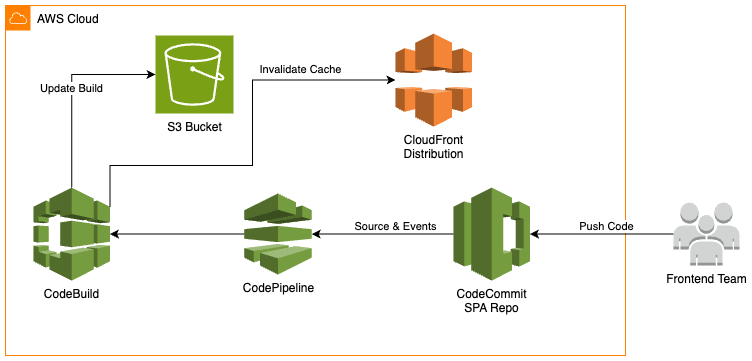
\includegraphics[width=0.9\linewidth]{immagini/infra/frontend_devops.png}%
    }
    \caption{Diagramma pipeline frontend}
    \label{auth_sequence}
\end{figure}





